\section{Introduction}

\subsection{LSST Data Management System}

To carry out this mission the Data Management System (DMS) performs the following major functions:

\begin{itemize}
\item Processes the incoming stream of images generated by the camera
  system during observing to produce transient alerts and to archive
  the raw images.

\item Roughly once per year, creates and archives a Data Release (``DR''),
  which is a static self-consistent collection of data products
  generated from all survey data taken from the date of survey
  initiation to the cutoff date for the Data Release. The data
  products (described in detail in the \DPDD), include measurements of 
  the properties (shapes, positions, fluxes, motions, etc.) of all detected
  objects, including those below the single visit sensitivity limit,
  astrometric and photometric calibration of the full survey object
  catalog, and limited classification of objects based on both their
  static properties and time-dependent behavior.  Deep coadded images
  of the full survey area are produced as well.

\item Periodically creates new calibration data products, such as bias
  frames and flat fields, that will be used by the other processing
  functions, as necessary to enable the creation of the data products above.

\item Makes all LSST data available through interfaces that utilize,
  to the maximum possible extent, community-based standards such as those
  being developed by the Virtual Observatory (``VO''), and facilitates user
  data analysis and the production of user-defined data products at Data
  Access Centers (``DAC'') and at external sites.
\end{itemize}

The overall architecture of the DMS is discussed in more detail in the Data Management System Design (\DMSD) document. The overall architecture of the DMS is shown in Figure~\ref{fig:DMS}.
\\

This document discusses the role of the Applications layer in the first three functions listed above (the functions involving \emph{science pipelines}).  The fourth is discussed separately in the SUI Conceptual Design Document (\SUI).

\begin{figure}
\centering
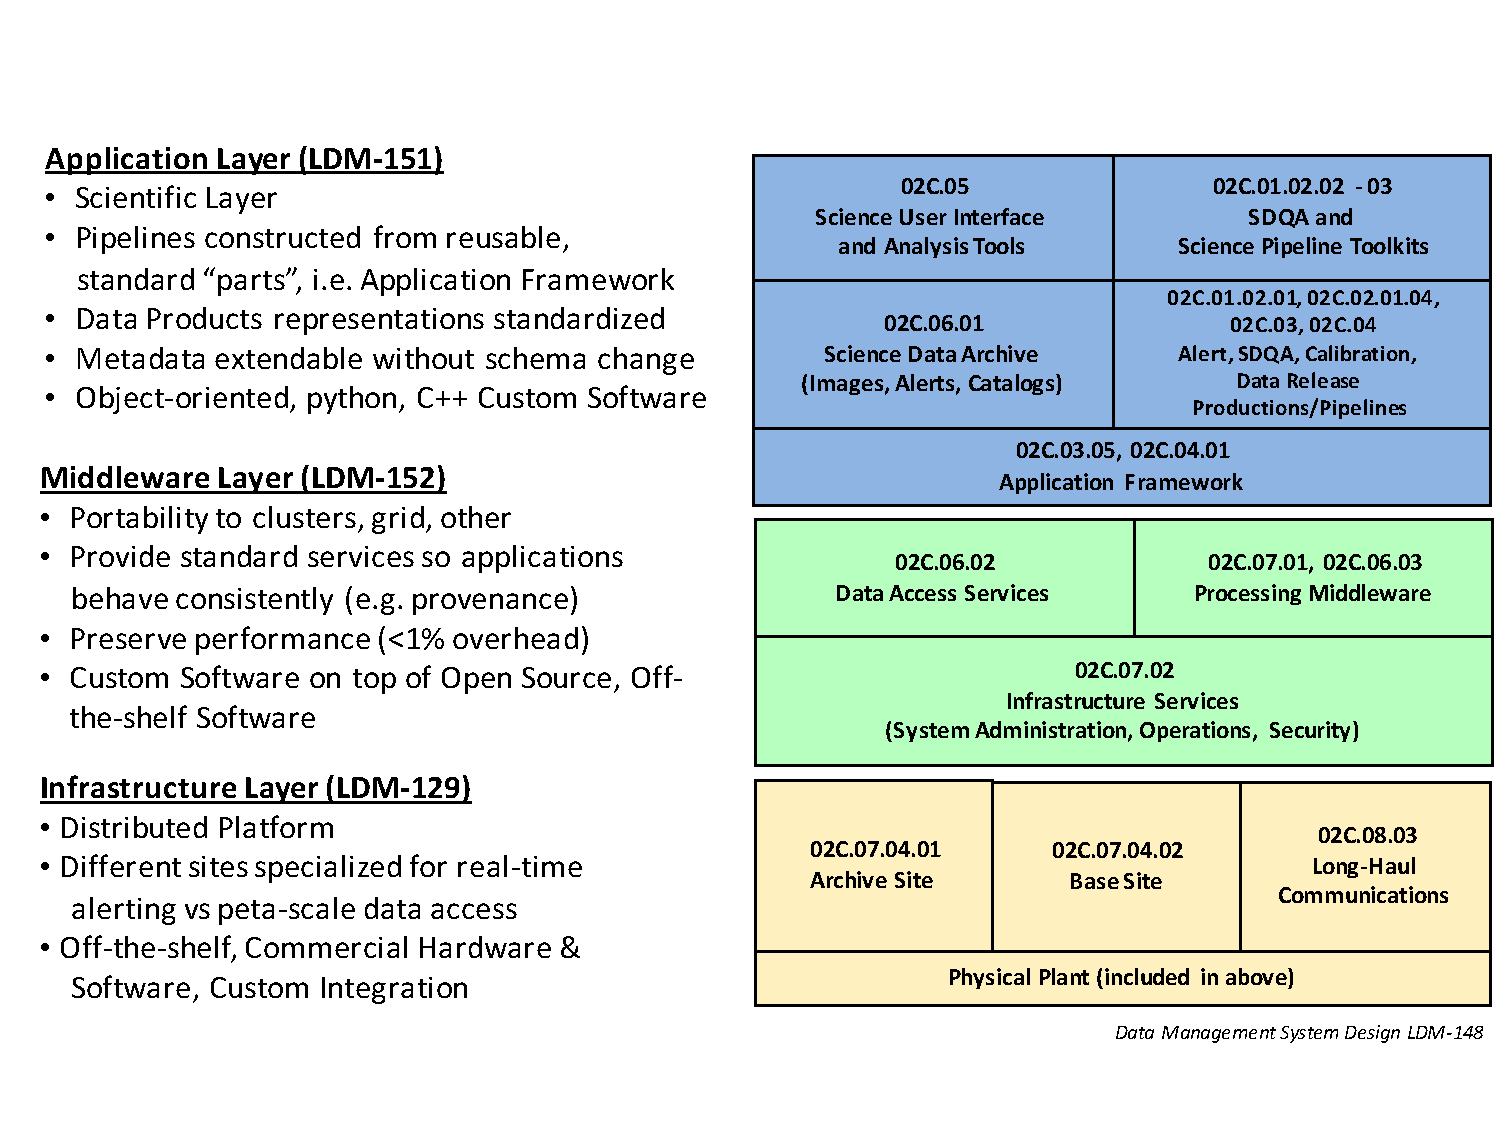
\includegraphics[angle=90,scale=0.70]{figures/DMS-Architecture.pdf}
\caption{Architecture of the Data Management System\label{fig:DMS}}
\end{figure}

\begin{figure}
%\includegraphics[angle=90,scale=0.70]{ApplicationLayerProductionsandPipelines.eps}
\centering
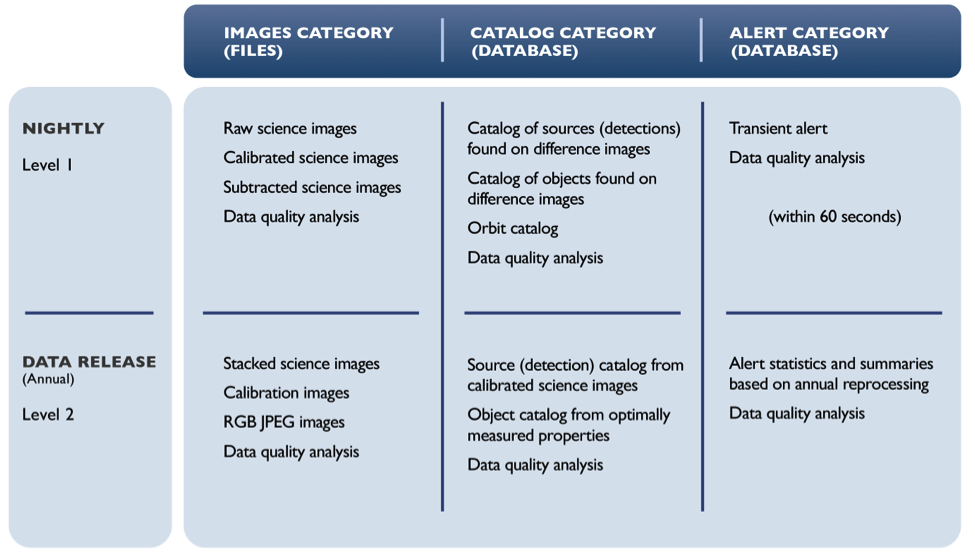
\includegraphics[angle=90]{figures/DataProductDelivarables.png}
\caption{Organization of LSST Data Products\label{fig:DP}}
\end{figure}

\subsection{Data Products}

The LSST data products are organized into three groups, based on their intended use and/or origin. The full description is provided in the Data Products Definition Document (\DPDD); we summarize the key properties here to provide the necessary context for the discussion to follow. 

\begin{itemize}
\item {\bf Level 1} products are intended to support timely detection and follow-up
  of time-domain events (variable and transient sources). They are generated by
  near-real-time processing the stream of data from the camera system during 
  normal observing.  Level 1 products are therefore continuously generated and / or
  updated every observing night. This process is of necessity highly
  automated, and must proceed with absolutely minimal human
  interaction.  In addition to science data products, a number of related
  Level 1 ``SDQA''\footnote{Science Data Quality Analysis} data products are generated
  to assess quality and to provide feedback to the Observatory Control System (OCS).

\item {\bf Level 2} products are generated as part of a Data Release, generally
  performed 
  yearly, with an additional data release for the first 6 months of survey data. 
  Level 2 includes data products for which extensive
  computation is required, often because they combine information from
  many exposures.  Although the steps that generate Level 2 products
  will be automated, significant human interaction may be required at
  key points to ensure the quality of the data.

\item {\bf Level 3} products are generated on any computing resources
  anywhere and then stored in an LSST Data Access Center. Often, but not
  necessarily, they will be generated by users of LSST using LSST software
  and/or hardware. LSST DM is required to facilitate the creation of
  Level 3 data products by providing suitable APIs, software components, and
  computing infrastructure, but will not by itself create any Level 3
  data products. Once created, Level 3 data products may be associated with
  Level 1 and Level 2 data products through database federation.
  Where appropriate, the LSST Project, with the agreement of the Level 3
  creators, may incorporate user-contributed Level 3 data product pipelines
  into the DMS production flow, thereby promoting them to Level 1 or 2.

\end{itemize}

\begin{note}{JFB comment:}
Should we mention intermediate data products as a category here, too?  Those will be an important part of the Pipeline descriptions that happen later in the document.
\end{note}

The organization of LSST Data Products is shown in Figure~\ref{fig:DP}.

Level 1 and Level 2 data products that have passed quality control
tests will be accessible to the public without restriction.
Additionally, the source code used to generate them will be made
available, and LSST will provide support for builds on selected
platforms.

\subsubsection{Data Units}

\begin{note}[TODO]
  This section still in outline form.
\end{note}

\begin{itemize}
  \item Source vs. Object
  \item Visit, CCD, Snap
  \item Tract, Patch
  \item Filters and object SEDs
\end{itemize}

\subsection{Science Pipelines Organization}

\begin{note}[TODO]
  This section still in outline form.  Expanded form should be short; I'm proposing we move the longer overviews that used to be in the introductions into the beginning of the sections for each Production, and shorten them to little more than a description of that Production's overview diagram.
\end{note}

\begin{itemize}
\item In sections (bla) we describe Alert Production, Calibration Product Production, and Data Release Production by decomposing them Pipelines.  Pipelines are not reusable; they occupy a specific place in a Production.
\item In section (bla) we describe the SDQA system, a set of smaller Productions as well as independent Pipelines within AP and DRP that verify the quality of the algoritms and data.
\item In section (bla) we say something with scope TBD about SUIT and enabling Level 3.
\item Pipelines are composed of reusable Algorithmic Components, which are described in section (bla).
\item Algorithmic Components rely on shared software primitives, described in section (bla).

\end{itemize}
